\documentclass[9pt]{article}

\setlength{\parindent}{0pt}
\usepackage{xltxtra}
\usepackage{hyperref}
\hypersetup{hidelinks}
\usepackage{url}
\urlstyle{tt}
\usepackage{xcolor}
\definecolor{CVBlue}{RGB}{23,110,191}
\usepackage{calc}
\usepackage{graphicx}
\usepackage{tikz}
\usetikzlibrary{calc}
\usepackage{fontspec}
\usepackage{xeCJK}
\usepackage{enumitem}
\CJKsetecglue{}

\setmainfont[
    Path = fonts/Main/,
    Extension = .otf,
    BoldFont = texgyretermes-bold.otf,
]{texgyretermes-regular.otf}

\setCJKmainfont[
    Path = fonts/hansans/,
    Extension = .ttf,
    BoldFont = NotoSansSC-Bold.ttf,
]{NotoSansSC-Regular.otf}

\usepackage{fontawesome}
\usepackage[
    a4paper,
    left=1.0cm,
    right=1.0cm,
    top=1.2cm,
    bottom=0.8cm,
    nohead
]{geometry}

\renewcommand{\baselinestretch}{1.15}

\usepackage{titlesec}
\setlist{noitemsep}
\setlist[itemize]{topsep=0.15em, leftmargin=*}

\titleformat{\section}
{\large\bfseries\raggedright}
{}{0em}{}
[{\color{CVBlue}\titlerule}]
\titlespacing*{\section}{0cm}{*1.0}{*0.6}

\begin{document}
\pagenumbering{gobble}

% 照片
\begin{tikzpicture}[remember picture, overlay] 
    \node[anchor = north east] at ($(current page.north east)+(-1.8cm,-0.5cm)$) {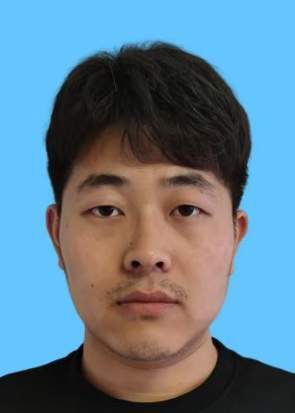
\includegraphics[height=2.8cm]{报名照片.jpg}};
\end{tikzpicture}

% 姓名
\centerline{\Large\bfseries{杜春龙}} 
\vspace{0.2em}
\centerline{\normalsize{\faPhone\ 136-3430-2571 \quad 
\faEnvelopeO\ \href{mailto:chunlongdu@stu.hrbnu.edu.cn}{chunlongdu@stu.hrbnu.edu.cn}}}

\vspace{0.5em}

% ===================== 科研成果综述 =====================
\centerline{\small
\textbf{科研成果概述：}已发表 SCI 二区论文 1 篇（第一作者，IF=4.1），
SCI 二区论文 1 篇（学生第二作者），
发明专利 1 项（实审中）。
研究方向聚焦遥感影像智能解译与语义分割模型设计。
}

% ===================== 教育背景 =====================
\section{\faGraduationCap\ 教育背景}

\textbf{哈尔滨师范大学} \hfill 测绘工程（硕士） \hfill 2023.09 -- 至今

\begin{itemize}
    \item GPA：3.78/4.0（专业前15\%）
    \item 研究方向：遥感影像语义分割、多尺度特征融合、频域特征建模、边界感知分割
    \item 毕业论文：基于几何上下文与频域融合的滑坡识别深度学习模型研究
\end{itemize}

\vspace{0.4em}

\textbf{长春工业大学} \hfill 软件工程（学士） \hfill 2019.09 -- 2023.06

\begin{itemize}
    \item GPA：3.46/4.0（专业前10\%）
    \item 核心课程：数据结构（92）、高等数学（90）、Python数据处理（91）
\end{itemize}

% ===================== 科研成果 =====================
\section{\faBook\ 科研成果}

\textbf{（一）已发表论文}

\begin{itemize}

\item \textbf{\textbf{Du}, Chunlong}, Qi S., Wan L., et al. 
GCF-Net: A Geometric Context and Frequency Domain Fusion Network for Landslide Segmentation in Remote Sensing Imagery. 
\textit{Remote Sensing}, 2026.  
（SCI 二区，IF=4.1，第一作者）  

\small{
针对滑坡边界模糊与尺度变化大的问题，提出几何上下文与频域融合双分支网络结构，提升复杂地形下分割精度。  
\textbf{本人贡献：}独立完成模型设计、代码实现、实验构建、消融分析及论文撰写。
}

\item Chen Y., Qi S., Wan L., \textbf{Du, Chunlong}, et al.  
HyM3S: Integrating Multiscale Spatial–Spectral Features With Sequence Modeling for Hyperspectral Classification.  
\textit{IEEE JSTARS}, 2025.  
（SCI 二区，IF=5.3，学生第二作者）

\small{
构建多尺度空间-光谱序列建模框架，实现高光谱地物分类精度提升。  
\textbf{本人贡献：}参与模型实验设计、结果分析与论文修改。
}

\end{itemize}

\vspace{0.3em}

\textbf{（二）专利}

融合几何上下文与频域多源特征的滑坡检测方法（中国发明专利，实审中）

% ===================== 科研经历 =====================
\section{\faFlask\ 科研经历}

\textbf{黑龙江省自然科学基金项目}（省部级）  
融合多源多时相遥感与深度学习的农作物精细分类与灾情识别方法  
核心成员 \hfill 2025.12 -- 2028.12

\begin{itemize}
    \item \textbf{研究背景：}复杂农业场景中存在类别混淆与时序特征表达不足问题
    \item \textbf{技术路线：}构建“光谱-纹理-时序”协同建模框架，融合多源遥感与深度网络
    \item \textbf{本人职责：}负责语义分割模型架构设计、多尺度特征融合模块改进、实验方案制定与性能评估
\end{itemize}

% ===================== 实践经历 =====================
\section{\faCogs\ 实践经历}

\textbf{基于启发式算法的智能装载系统}  
开发成员 \hfill 2022.08 -- 2022.12

\begin{itemize}
    \item 基于启发式优化算法实现装载方案自动生成
    \item 负责数据库设计与核心模块开发
    \item 优化查询逻辑，提高系统响应效率
\end{itemize}

% ===================== 专业技能 =====================
\section{\faLaptop\ 专业技能}

\begin{itemize}
    \item \textbf{深度学习框架：}熟练使用 PyTorch、TensorFlow，能够独立搭建语义分割与特征融合模型
    \item \textbf{编程能力：}Python（科研建模）、C、Java
    \item \textbf{科研工具：}LaTeX、EndNote、Zotero，熟悉SCI投稿与审稿流程
    \item \textbf{英语能力：}CET-6，具备英文论文写作与学术交流能力
\end{itemize}

\end{document}
